% SeasonSafe -- IEEE conference paper source (AMLBT, Goa Institute of Management).
% Build: pdflatex seasonsafe.tex (twice). Overleaf: upload this file and figures/ into a copy of the course template.
% DRAFT generated with AI assistance on 19 Nov 2026 -- see Section IX-A. The team must review, rewrite and own the text.
\documentclass[conference]{IEEEtran}
\usepackage{amsmath,amssymb}
\usepackage{graphicx}
\usepackage{booktabs}
\usepackage{url}
\usepackage[hidelinks]{hyperref}
\graphicspath{{figures/}}

\begin{document}

\title{SeasonSafe: Do E-Commerce Purchase-Score Cutoffs Survive a Change in Shopping Patterns?}

% TODO(team): add every team member, student ID and institutional e-mail as in the course template.
\author{\IEEEauthorblockN{Yashwanth M}
\IEEEauthorblockA{Goa Institute of Management, Big Data Analytics\\
Student ID: B2026161}}

\maketitle

\begin{abstract}
A purchase score helps a retailer only when it supports a workable decision, such as which sessions
a limited sales or service team should attend to. We test whether a score cutoff calibrated to select
10\% of October sessions still selects 10\% in November and December, using 12,330 sessions from the
UCI Online Shoppers Purchasing Intention dataset. Models trained on February--September were chosen
on October and evaluated on the two held-out months. The frozen cutoff selected 249 sessions against a
November budget of 299 and 182 against a December budget of 172. Ranking within each month met the
budget by construction without a clear precision gain. Post-hoc checks qualify these numbers. The
month indicator is unseen for every evaluation row, and removing it turns December's overflow into an
underflow. Re-estimating the cutoff on resampled October data yields a 95\% range of 127--208 December
selections. A ``new visitors first'' rule nearly matches the model's top-decile precision. The robust
conclusion is that a frozen probability cutoff does not hold a workload steady under traffic-mix
shift. Capacity, probability reliability and feature availability must be monitored separately.
\end{abstract}

\begin{IEEEkeywords}
E-commerce, purchase intention, temporal validation, dataset shift, capacity constraints, probability calibration
\end{IEEEkeywords}

\section{Introduction}
Online retailers increasingly score live sessions for purchase propensity and act on the highest
scores: a chat agent, a call-back, a targeted banner or a sales follow-up. Each action consumes a
scarce resource. The operational question is therefore not only ``how well does the model rank
shoppers?'' but also ``how many sessions will the rule send to the team next month?''.

A common implementation freezes a probability threshold chosen on recent data and applies it
going forward. That rule silently assumes the score distribution is stable. Seasonal campaigns,
new traffic sources and changes in the mix of new and returning visitors can each move scores, so a
cutoff tuned for one month may starve or flood the team in the next. Concept-drift research has long
documented such failures for model accuracy \cite{b7,b8}. Their consequence for \emph{workload} is rarely
measured in purchase-intention studies.

\subsection{Scope and objectives}
SeasonSafe audits that consequence on public data. The objectives are to: (i) measure how far a frozen
October cutoff misses a 10\% selection budget in November and December; (ii) compare it with an offline
monthly top-10\% rule; (iii) check whether predicted buyer volumes remain reliable; (iv) quantify how
much the results depend on information that would not exist when a visitor arrives; and (v) diagnose
\emph{why} the cutoff drifts and whether a simpler rule would do as well. The study uses historical
outcomes and makes no claim about incremental sales caused by any intervention.

\section{Related Work}
Sakar \emph{et al.} \cite{b2} introduced the dataset and combined aggregated session features with
sequential clickstream models (MLP and LSTM) for real-time purchase and abandonment prediction. Baati
and Mohsil \cite{b3} predicted purchase intention from session and user information available when a
visitor connects. Arrival-time prediction is therefore not new. Moe and Fader \cite{b9} modelled conversion as
the interplay of visit frequency and a purchasing threshold that changes with experience, which motivates
treating visitor history (new versus returning) as a primary signal.

Work on dataset shift \cite{b10} and concept-drift adaptation \cite{b7} distinguishes covariate shift from changes in
the outcome relationship and recommends monitoring both. Rabanser \emph{et al.} \cite{b8} show that detecting
shift is feasible with simple two-sample tests even when its effect on accuracy is unknown. On the
probability side, Platt scaling \cite{b11} and isotonic regression \cite{b12} are standard recalibration maps, and
Niculescu-Mizil and Caruana \cite{b13} show that tree ensembles and boosting are often poorly calibrated.
Kaufman \emph{et al.} \cite{b14} formalise leakage as using information that would not be available at
prediction time, which is our concern with completed-session variables such as PageValues.

Table~\ref{tab:rw} positions SeasonSafe. Its contribution is narrow and operational. It connects a frozen
decision rule to capacity error, buyer-volume reliability and feature-timing limits in one time-ordered
audit, and it tests that audit against encoding artefacts, cutoff noise and rule baselines. It does not
propose a new learning algorithm.

\begin{table}[t]
\caption{Positioning against prior work}\label{tab:rw}
\centering\footnotesize
\begin{tabular}{@{}p{1.25cm}p{1.6cm}p{1.45cm}p{2.6cm}@{}}
\toprule
Work & Data & Validation & Decision / capacity view\\
\midrule
\cite{b2} & UCI + clickstream & Random split & Real-time prediction; no budget\\
\cite{b3} & UCI, arrival info & Random split & Early prediction; no budget\\
\cite{b7,b8} & Generic streams & Temporal & Drift detection; accuracy focus\\
\textbf{Ours} & UCI, arrival proxies & Train Feb--Sep, select Oct, test Nov--Dec & Frozen vs.\ monthly top-$k$; capacity error, buyer-volume reliability, rule baselines\\
\bottomrule
\end{tabular}
\end{table}

\section{Data}
The dataset holds 12,330 sessions from one online retailer over one year, each from a different user
\cite{b1}; 1,908 (15.47\%) end in a purchase. \texttt{Revenue} is a binary purchase flag, not an amount.
There are no January or April sessions. Months are highly unequal: May supplies 3,364 sessions and
October only 549 (Fig.~\ref{fig:rates}).

\textbf{Primary (arrival-context) features} are Month, OperatingSystems, Browser, Region, TrafficType,
VisitorType, Weekend and SpecialDay. Their availability at arrival is assumed, not verified. Coded
categories are treated as nominal. \textbf{Retrospective features} (page counts, durations,
BounceRates, ExitRates) summarise the completed session. PageValues is transaction-related and its
point-in-time construction is undocumented. Excluding it is a conservative choice, not proof of
leakage \cite{b14}.

The 125 exact duplicate rows are retained in the primary analysis because no session identifier proves
they are repeated events; a pre-specified sensitivity removes them. Preprocessing (median imputation,
standardisation, one-hot encoding with unknown categories ignored) is fitted on training rows only \cite{b4}.

\begin{figure}[t]
\centering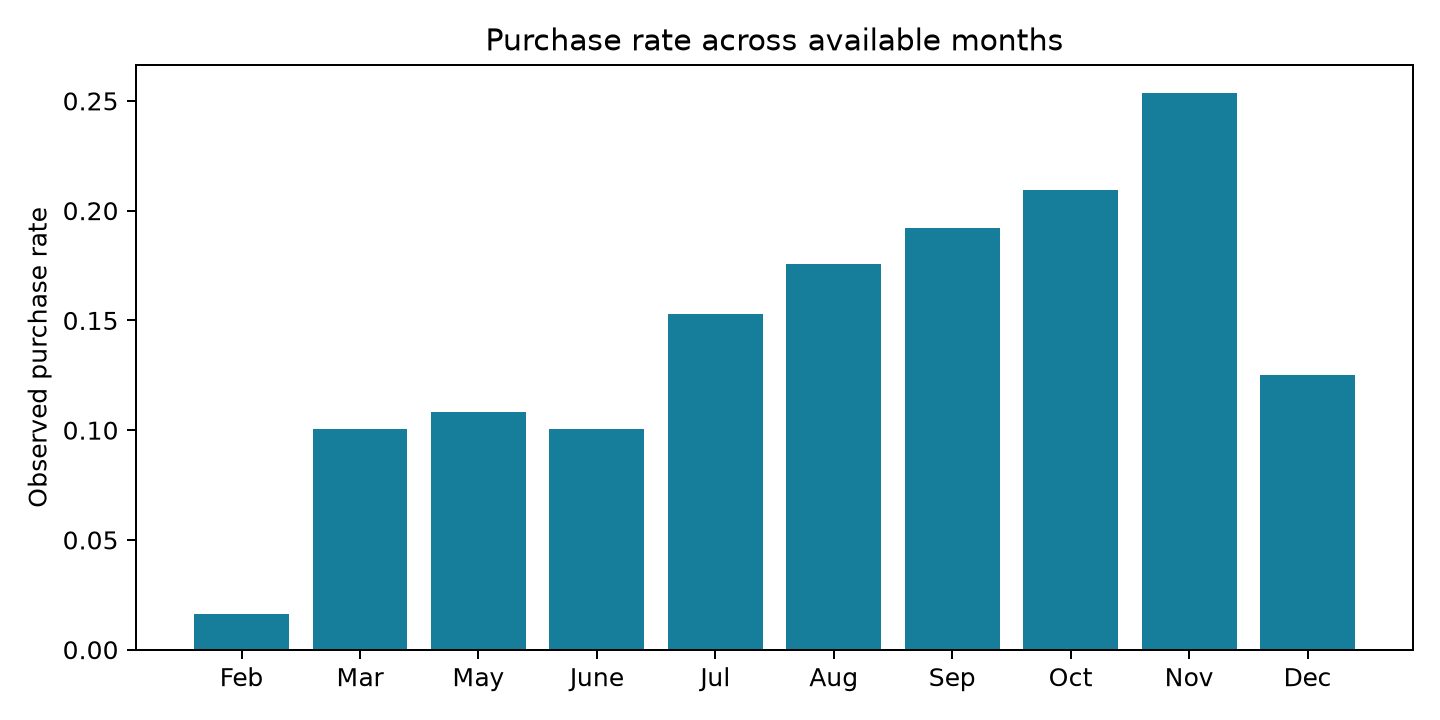
\includegraphics[width=0.92\columnwidth]{01_monthly_purchase_rates.png}
\caption{Observed purchase rate by month. Rates rise from 1.6\% (Feb) to 25.4\% (Nov) and fall to 12.5\% (Dec).}
\label{fig:rates}
\end{figure}

\section{Methodology}
\subsection{Chronological design}
Training uses February--September (7,056 sessions, 817 purchases); October (549/115) selects the model
and sets the cutoff; November (2,998) and December (1,727) are held out. All choices were saved in a
decision manifest before test outcomes were computed.

\subsection{Models}
Three scikit-learn \cite{b5} classifiers are fitted per feature set: L2 logistic regression ($C=1$); a random
forest \cite{b15} (200 trees, minimum leaf 10, $\sqrt{p}$ features); and histogram gradient boosting \cite{b16}
(150 iterations, 15 leaves, L2 penalty 1, no early stopping). The primary model is chosen \emph{within the
arrival-context family} by October average precision (AP), with the Brier score as tie-break. Seed: 161.

\subsection{Selection policies}
Let $s_i$ be the score of session $i$ and $B=\lfloor 0.1\,n\rfloor$ the monthly budget for $n$ sessions.
The \emph{fixed policy} freezes the October cutoff
\begin{equation}
\tau = s^{\mathrm{Oct}}_{(B_{\mathrm{Oct}})},\qquad S_{\mathrm{fixed}}=\{i : s_i \ge \tau\},
\end{equation}
where $s_{(k)}$ is the $k$-th largest score. The \emph{batch policy} selects exactly the $B$ highest
scores in each month with seeded random tie-breaking. It is an offline reference, because a live
queue cannot see the month's later arrivals. Capacity error is $|S|-B$.

\subsection{Evaluation metrics}
Business metrics: selected count, unused capacity $U=\max(0,B-|S|)$, overflow $O=\max(0,|S|-B)$,
precision $=\sum_{i\in S}y_i/|S|$, and predicted minus observed buyers in $S$. Accuracy is unsuitable at a
15\% base rate, so diagnostics use AP (preferred to ROC under imbalance \cite{b17}), ROC-AUC, Brier score and log
loss. Random targeting's expected precision equals the month's base rate. A constant model at the
training prevalence is the probability baseline. Precision differences between policies receive approximate
95\% paired-bootstrap intervals \cite{b18} (500 resamples), conditional on the fitted model.

\subsection{Post-hoc analyses}
After the held-out results were seen, we added: an ablation removing Month and SpecialDay; rule
baselines that rank by training purchase rate per VisitorType and TrafficType; a 2,000-resample bootstrap of
October to propagate cutoff uncertainty; a seed sweep (161--170) and training-only expanding-window
tuning; Platt and isotonic recalibration fitted on October; feature drift measured by the population
stability index
\begin{equation}
\mathrm{PSI}=\sum_j (a_j-e_j)\ln(a_j/e_j),
\end{equation}
over category shares $e_j$ (reference) and $a_j$ (target); permutation importance; and a label-free
rolling policy that sets each month's cutoff from the previous month's scores. These analyses are labelled
post-hoc throughout and do not replace the locked result.

\section{Results}
\subsection{Model selection}
In October, boosting (AP 0.2502) narrowly beat logistic regression (0.2488) and the random forest
(0.2372). The 0.0014 margin is far smaller than any plausible sampling error on 549 sessions. Held-out
ROC-AUC was 0.597 (Nov) and 0.638 (Dec), showing limited separation.

\subsection{Capacity and buyer concentration}
Table~\ref{tab:policy} gives the primary result. The frozen cutoff left 50 November slots (16.7\%) unused
and exceeded December's budget by 10 (5.8\%). The batch policy met both budgets by construction.
Paired-bootstrap intervals for batch-minus-fixed precision were $[-4.11,+0.97]$ points in November and
$[-1.99,+2.33]$ in December. Both include zero, so neither policy shows a precision advantage.

\begin{table}[t]
\caption{Primary policy results, 10\% budget (locked analysis)}\label{tab:policy}
\centering\footnotesize
\begin{tabular}{@{}llrrrr@{}}
\toprule
Month & Policy & Budget & Selected & Buyers & Precision\\
\midrule
Oct (val.) & Fixed = batch & 54 & 54 & 11 & 20.37\%\\
Nov & Fixed Oct cutoff & 299 & 249 & 85 & 34.14\%\\
Nov & Monthly top 10\% & 299 & 299 & 98 & 32.78\%\\
Dec & Fixed Oct cutoff & 172 & 182 & 43 & 23.63\%\\
Dec & Monthly top 10\% & 172 & 172 & 40 & 23.26\%\\
\bottomrule
\end{tabular}
\end{table}

\begin{figure}[t]
\centering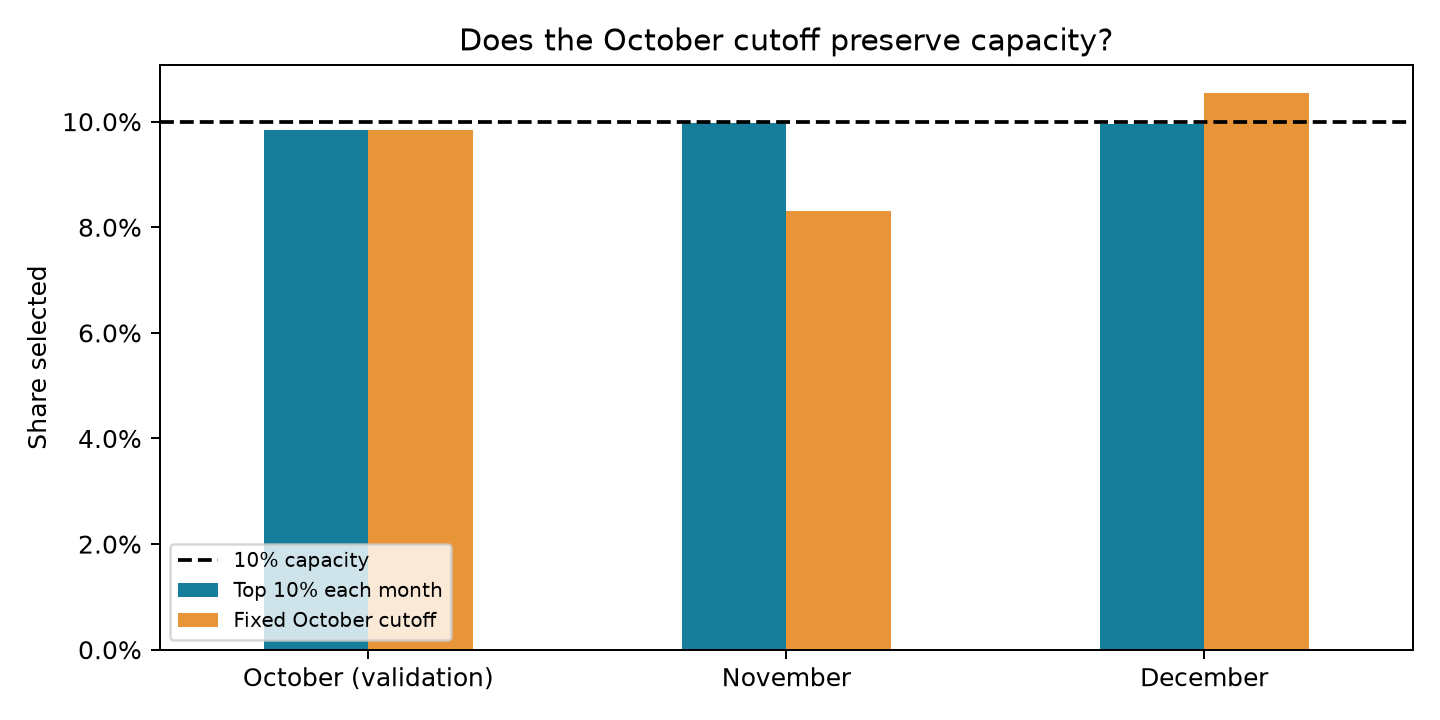
\includegraphics[width=0.92\columnwidth]{02_capacity_drift.png}
\caption{Share selected by each policy. The dashed line is the 10\% target.}
\label{fig:drift}
\end{figure}

\subsection{Probability reliability}
Among December's 172 top-ranked sessions the model predicted 58.65 buyers; 40 purchased, an
overestimate of 46.6\%. November's 299 predicted 100.47 against 98 observed (Fig.~\ref{fig:rel}).
Recalibrating on October (post-hoc) \cite{b6} lowered the November Brier score from 0.1970 to 0.1874 (Platt) but
raised December's from 0.1089 to 0.1138. October's base rate (20.9\%) lies between November's (25.4\%) and
December's (12.5\%), so no single static map fits both months.

\begin{figure}[t]
\centering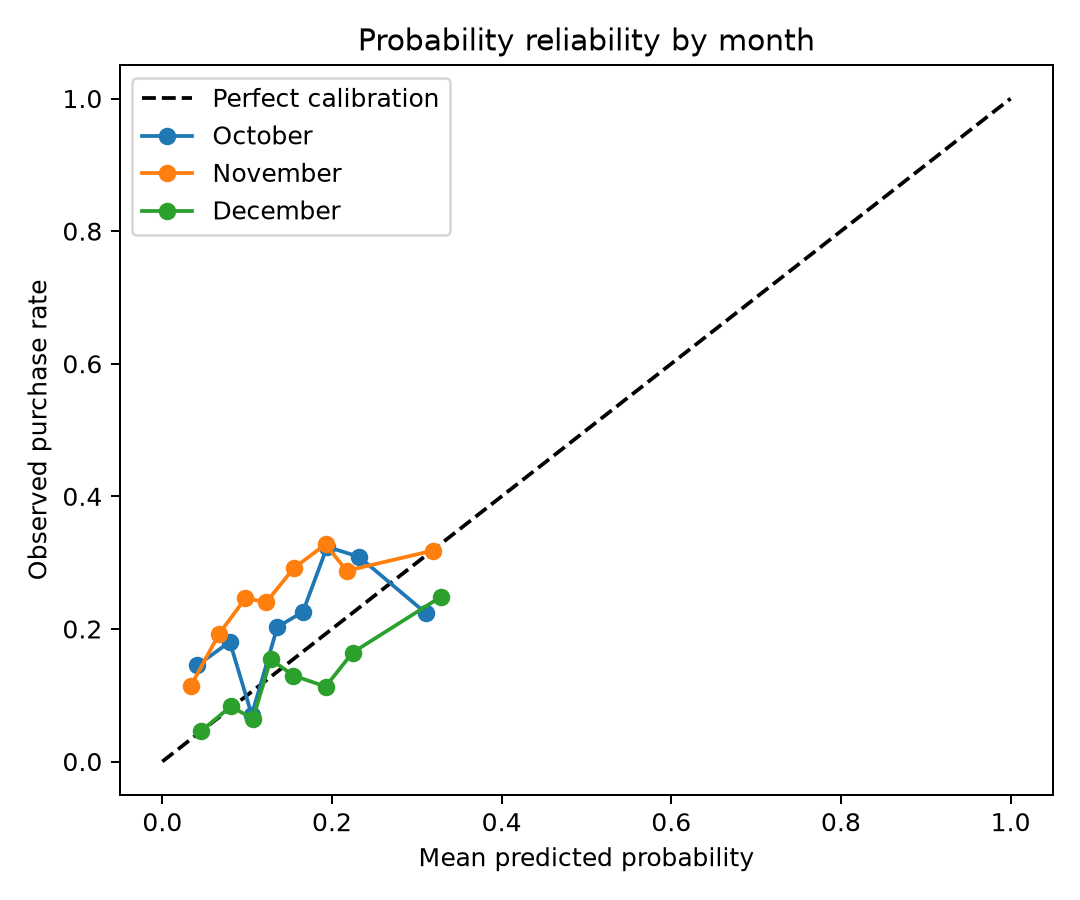
\includegraphics[width=0.85\columnwidth]{03_reliability.png}
\caption{Reliability diagrams (quantile bins) by month for the primary model.}
\label{fig:rel}
\end{figure}

\subsection{Feature availability}
Holding the boosting algorithm fixed, pooled held-out AP and ROC-AUC rise from 0.269/0.600 with
arrival-context proxies to 0.327/0.677 with completed-session behaviour and 0.651/0.824 when PageValues is
added. The stronger results describe information available only after the session, not at arrival.

\subsection{Robustness of the capacity finding (post-hoc)}
\emph{Unseen Month.} Because training ends in September, the Month categories of every validation and
test row are unseen. Their one-hot columns are all zero, an input pattern no training row had.
SpecialDay is non-zero only in February and May. Permutation importance for both features is exactly
zero from October onwards. They contribute nothing to ranking but still shift the score level.
Table~\ref{tab:abl} shows the consequence. Removing Month barely changes AP, yet December's frozen-cutoff
selection falls from 182 to 139 (boosting) or 105 (logistic). The overflow becomes an underflow.

\begin{table}[t]
\caption{Ablation, boosting, 10\% budget (post-hoc)}\label{tab:abl}
\centering\footnotesize
\begin{tabular}{@{}lrrrr@{}}
\toprule
Features & Oct AP & Nov sel./299 & Dec sel./172 & Dec AP\\
\midrule
Primary (8 features) & 0.250 & 249 & 182 & 0.194\\
$-$ Month & 0.252 & 232 & 139 & 0.200\\
$-$ Month, SpecialDay & 0.242 & 215 & 128 & 0.199\\
\bottomrule
\end{tabular}
\end{table}

\emph{Cutoff noise.} Re-estimating $\tau$ on 2,000 bootstrap resamples of October gives 95\% ranges
of 199--301 selected sessions in November and 127--208 in December. November under-fills in 96\% of
resamples, while December over-fills in only 80\%. Across target budgets from 2\% to 30\%, the
December error changes sign between the 10\% and 12\% targets (Fig.~\ref{fig:curve}).

\emph{Model choice and seeds.} Boosting won in every seed from 161 to 170. Had logistic regression won the
0.0014 race, the frozen cutoff would have selected 236 (Nov) and 183 (Dec). Training-only tuning did not
improve October AP and still produced 175--229 November and 162--167 December selections.

\begin{figure}[t]
\centering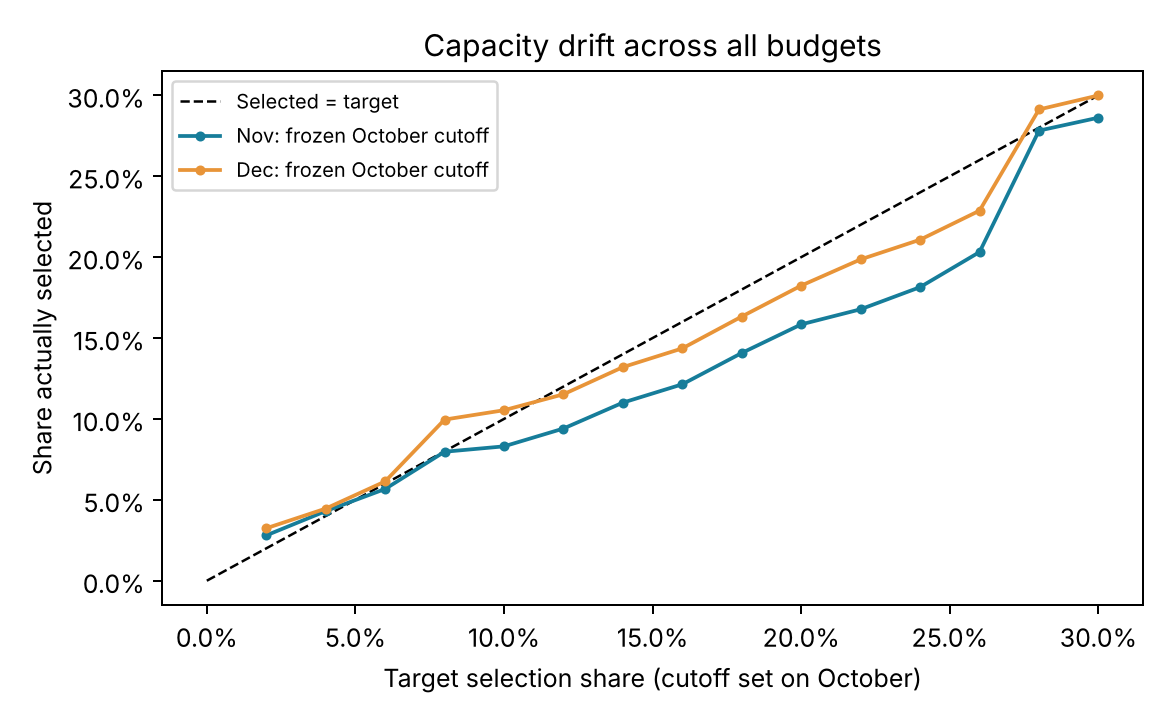
\includegraphics[width=0.92\columnwidth]{04_capacity_curve.png}
\caption{Share selected by the frozen October cutoff for every target budget (post-hoc).}
\label{fig:curve}
\end{figure}

\subsection{Why the cutoff drifts and what the model learned (post-hoc)}
TrafficType shows by far the largest shift. Types 4 and 5 (17\% of October traffic) almost vanish after
October, while types 8 and 10, absent in October, reach about 12\% of sessions. The new-visitor share moves
from 22.6\% to 14.0\% to 19.4\%. The frozen cutoff admits 40--51\% of new visitors but only about 1\% of
returning visitors (Fig.~\ref{fig:vt}), so the new-visitor share largely sets the selected volume.
Permutation importance ranks TrafficType and VisitorType highest.

Simple rules are close competitors (Fig.~\ref{fig:rules}). ``New visitors first, random within group''
reaches 30.4\% top-decile precision in November and 23.8\% in December against the model's 32.8\% and
23.3\%. A TrafficType purchase-rate rule wins November (34.1\%) but fails in December (16.9\%). A
label-free rolling cutoff using November's score quantile selected 205 sessions in December, worse than
the frozen cutoff, because the traffic mix moved in the opposite direction.

\begin{figure}[t]
\centering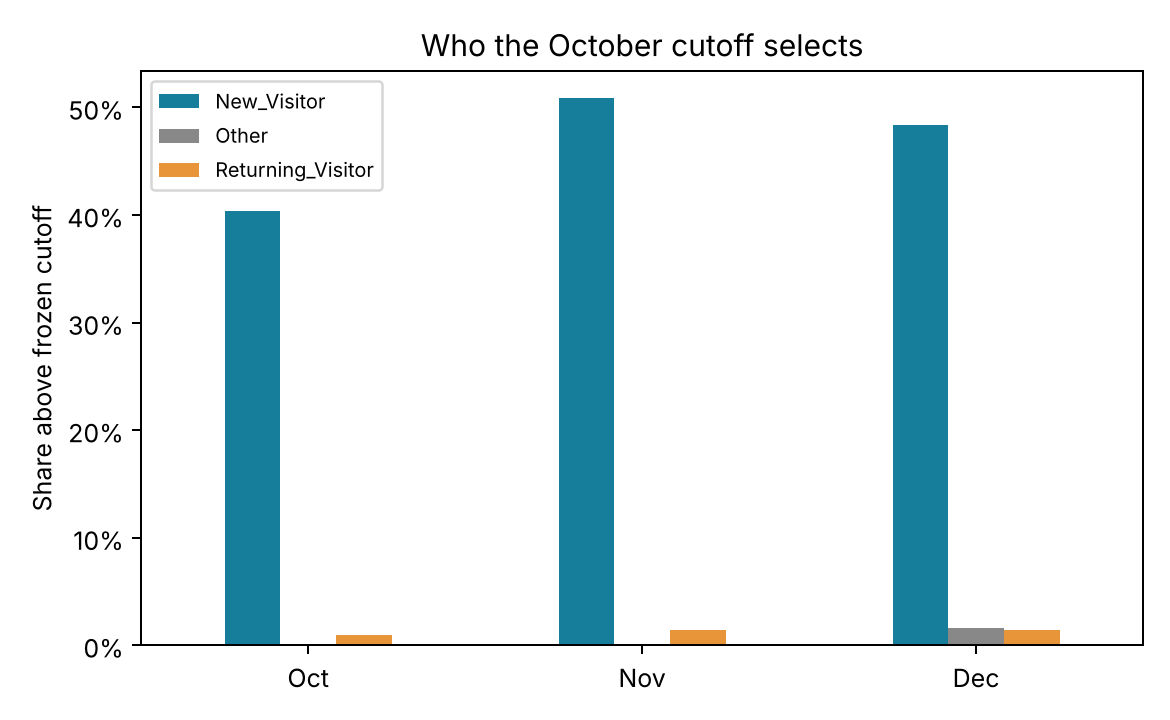
\includegraphics[width=0.92\columnwidth]{07_selection_by_visitor_type.png}
\caption{Share of each visitor type above the frozen October cutoff (post-hoc).}
\label{fig:vt}
\end{figure}

\begin{figure}[t]
\centering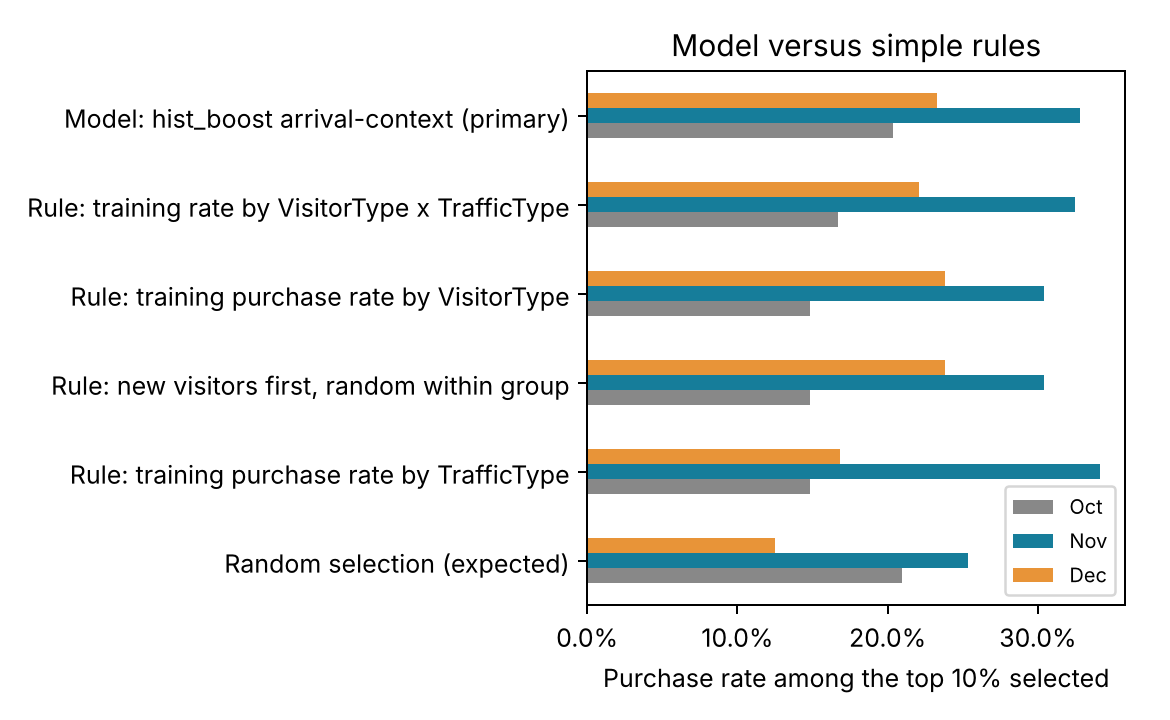
\includegraphics[width=0.92\columnwidth]{06_rule_baselines.png}
\caption{Top-10\% precision: model versus simple rules and random selection (post-hoc).}
\label{fig:rules}
\end{figure}

\subsection{Duplicate sensitivity (pre-specified)}
Removing the 125 identical rows and repeating the full protocol, the frozen cutoff selected 206 of 298
(November) and 129 of 170 (December). December again reverses from overflow to underflow.

\section{Discussion}
\textbf{What is robust.} In every variant, a probability cutoff frozen on one month failed to hold the
intended workload in later months, by up to a sixth of the budget. This matters to any team that
staffs against a score threshold. \textbf{What is not robust.} The direction and size of the error
depend on the unseen-month encoding, duplicate handling, the budget level, the algorithm and cutoff
estimation noise. A claim such as ``December overloads the team by 6\%'' would overstate the evidence.

\textbf{Business relevance.} The problem is an operational control problem, not just a modelling one.
A capacity-safe design would set a volume rule (top-$k$ per arrival window) and monitor probability
reliability separately, with recent labels. A frozen probability threshold delivers neither guarantee.
Under an assumed cost ratio $r$ of one overflow session to one idle slot, the mismatch cost $U+rO$ was 50
idle-slot units in November regardless of $r$, and $10r$ in December. Without real cost data this
illustrates the trade-off; it does not estimate money.

\textbf{Technical quality.} With arrival-time proxies the model is weak (AUC about 0.6) and close to a
visitor-type rule. The large gains from completed-session features and PageValues are not available at
arrival. Monitoring feature drift (PSI on TrafficType and VisitorType) would have flagged the shift
before outcomes arrived \cite{b8}. Calibration of boosted trees is unstable across months \cite{b13}, and a static
recalibration helps one month while hurting the other.

\textbf{Limitations.} One retailer and one year, at monthly resolution, with no timestamps, so a live
queue cannot be simulated. There are no treatment labels, so purchase propensity is not benefit from an
intervention. The 10\% budget is an assumption. The bootstrap intervals ignore temporal correlation and
model selection. All post-hoc analyses were chosen after seeing test outcomes and are explanatory, not
confirmatory.

\section{Conclusion}
A purchase-score cutoff frozen in October did not preserve a 10\% workload in November or December.
The miss is real, but its direction and size are fragile. Arrival-context models ranked shoppers only
modestly and performed close to a ``new visitors first'' rule. Before deploying purchase scores,
retailers should (i) control volume with an explicit top-$k$ rule per arrival window, (ii) monitor
traffic-mix drift and buyer-volume calibration separately, and (iii) verify which features truly exist
at decision time. Future work should use timestamped clickstreams to simulate a live queue, and
randomised interventions to estimate uplift rather than propensity.

\section{Reproducibility}
Code, the source and cleaned data, every result table and figure, and tests are available at
\url{https://github.com/YashwanthPb/SeasonSafe}. Install the pinned versions in
\texttt{requirements\_verified.txt} (Python 3.13/3.14, scikit-learn 1.9.0, pandas 3.0.5, NumPy 2.5.1). Then
run \texttt{experiment.py} (primary), \texttt{experiment.py --dedup} (sensitivity) and
\texttt{extended\_analysis.py} (post-hoc). A re-run reproduced every published table to within $10^{-12}$.
The decision manifest records the seed, cutoffs, versions and data SHA-256. Data: CC BY 4.0 \cite{b1}.

\subsection{AI Use Declaration}
ChatGPT assisted with topic refinement, the experimental protocol, the original code, documentation and
report drafting. Claude Code (Anthropic) assisted with the repository audit, the extended post-hoc analyses,
tests and this LaTeX draft. All empirical values were computed by code from the dataset and rechecked
against saved predictions. AI-generated text and code are substantial. Compliance with the course limit of
below 20\% has not been established; see \texttt{AI\_USE\_LOG.md}.
% TODO(team): replace with your own declaration after rewriting the paper yourselves.

\begin{thebibliography}{00}
\bibitem{b7} J. Gama, I. \v{Z}liobait\.{e}, A. Bifet, M. Pechenizkiy, and A. Bouchachia, ``A survey on concept drift adaptation,'' \emph{ACM Comput. Surv.}, vol. 46, no. 4, art. 44, 2014, doi: 10.1145/2523813.
\bibitem{b8} S. Rabanser, S. G\"unnemann, and Z. Lipton, ``Failing loudly: An empirical study of methods for detecting dataset shift,'' in \emph{Adv. Neural Inf. Process. Syst. 32}, 2019, pp. 1396--1408.
\bibitem{b2} C. O. Sakar, S. O. Polat, M. Katircioglu, and Y. Kastro, ``Real-time prediction of online shoppers' purchasing intention using multilayer perceptron and LSTM recurrent neural networks,'' \emph{Neural Comput. Appl.}, vol. 31, pp. 6893--6908, 2019, doi: 10.1007/s00521-018-3523-0.
\bibitem{b3} K. Baati and M. Mohsil, ``Real-time prediction of online shoppers' purchasing intention using random forest,'' in \emph{Artificial Intelligence Applications and Innovations}, IFIP AICT, vol. 583, 2020, pp. 43--51, doi: 10.1007/978-3-030-49161-1\_4.
\bibitem{b9} W. W. Moe and P. S. Fader, ``Dynamic conversion behavior at e-commerce sites,'' \emph{Manage. Sci.}, vol. 50, no. 3, pp. 326--335, 2004, doi: 10.1287/mnsc.1040.0153.
\bibitem{b10} J. Qui\~nonero-Candela, M. Sugiyama, A. Schwaighofer, and N. D. Lawrence, Eds., \emph{Dataset Shift in Machine Learning}. Cambridge, MA, USA: MIT Press, 2009.
\bibitem{b11} J. Platt, ``Probabilistic outputs for support vector machines and comparisons to regularized likelihood methods,'' in \emph{Advances in Large Margin Classifiers}. Cambridge, MA, USA: MIT Press, 1999, pp. 61--74.
\bibitem{b12} B. Zadrozny and C. Elkan, ``Transforming classifier scores into accurate multiclass probability estimates,'' in \emph{Proc. 8th ACM SIGKDD}, 2002, pp. 694--699.
\bibitem{b13} A. Niculescu-Mizil and R. Caruana, ``Predicting good probabilities with supervised learning,'' in \emph{Proc. 22nd ICML}, 2005, pp. 625--632.
\bibitem{b14} S. Kaufman, S. Rosset, C. Perlich, and O. Stitelman, ``Leakage in data mining: Formulation, detection, and avoidance,'' \emph{ACM Trans. Knowl. Discov. Data}, vol. 6, no. 4, art. 15, 2012, doi: 10.1145/2382577.2382579.
\bibitem{b1} C. Sakar and Y. Kastro, ``Online Shoppers Purchasing Intention Dataset,'' UCI Machine Learning Repository, 2018, doi: 10.24432/C5F88Q.
\bibitem{b4} scikit-learn developers, ``Common pitfalls and recommended practices,'' scikit-learn documentation. [Online]. Available: https://scikit-learn.org/stable/common\_pitfalls.html
\bibitem{b5} F. Pedregosa \emph{et al.}, ``Scikit-learn: Machine learning in Python,'' \emph{J. Mach. Learn. Res.}, vol. 12, pp. 2825--2830, 2011.
\bibitem{b15} L. Breiman, ``Random forests,'' \emph{Mach. Learn.}, vol. 45, no. 1, pp. 5--32, 2001.
\bibitem{b16} G. Ke \emph{et al.}, ``LightGBM: A highly efficient gradient boosting decision tree,'' in \emph{Adv. Neural Inf. Process. Syst. 30}, 2017, pp. 3146--3154.
\bibitem{b17} T. Saito and M. Rehmsmeier, ``The precision-recall plot is more informative than the ROC plot when evaluating binary classifiers on imbalanced datasets,'' \emph{PLoS ONE}, vol. 10, no. 3, e0118432, 2015.
\bibitem{b18} B. Efron and R. J. Tibshirani, \emph{An Introduction to the Bootstrap}. New York, NY, USA: Chapman \& Hall, 1993.
\bibitem{b6} scikit-learn developers, ``Probability calibration,'' scikit-learn documentation. [Online]. Available: https://scikit-learn.org/stable/modules/calibration.html
\end{thebibliography}

\end{document}
